\documentclass{CFD2010paper}

%\usepackage{graphicx}
\usepackage[pdftex]{graphicx,color}

\title{PARAMETRIC STUDY OF A MULTISCALE FLUIDIC SYSTEM\newline
USING A HYBRID CFD-MD APPROACH}

\author{Soon-Heum Ko$^{\dag}$, Nayong Kim$^{\dag}$, Dimitris E. Nikitopoulos$^{\dag\dag}$, Dorel Moldovan$^{\dag\dag}$ and Shantenu Jha$^{{\dag},*}$}

\heading{S.-H. Ko, N. Kim, D. Nikitopoulos, D. Moldovan, and S. Jha}

\address{
$^{\dag}$Center for Computation and Technology,\\
Louisiana State University, 216 Johnston Hall, Baton Rouge, LA 70803\\
e-mail: \{sko,nykim,sjha\}@cct.lsu.edu
\\
$^{\dag\dag}$Department of Mechanical Engineering,\\
Louisiana State University, Baton Rouge, LA 70803\\
e-mail: \{meniki,moldovan\}@me.lsu.edu
\\
$^{*}$Contact Author}


\keywords{CFD (Computational Fluid Dynamics), MD (Molecular Dynamics), Hybrid CFD-MD Approach, Pseudo Compressibility, LAMMPS}

\abstract{
Hybrid continuum fluid dynamics (CFD) molecular dynamics (MD) simulation methodology is a reliable simulation approach capable of accurately describing the flow at both molecular and macroscopic scales. In this approach the continuum and molecular domains are coupled through an overlap region that facilitates the exchange of information between them forcing the two descriptions to match each other by imposing constrained molecular dynamics and boundary conditions based on time and spatial averaging of relevant physical properties in the overlap region. Despite the recent developments reported in literature, most of them tested against small idealized pure atomistic simulations, there are a few methodological and implementation issues that need further refinement, testing and validation. Specifically, two sets of issues need further clarification: (1) identify the limits and the optimal conditions for a hybrid implementation (e.g., size of the overlap region, sampling time for atomistic averaging, etc.), (2) asses the feasibility of applying the hybrid approach to unsteady flow problems. Using a hybrid CFD-MD implementation we address these issues by focusing on two classical flow problems: the steady Couette flow and the unsteady Stokes boundary layer flow. An in-house incompressible Navier-Stokes CFD code and the LAMMPS MD package are used as baseline codes in our hybrid scheme. We begin by presenting the results of the stationary flow simulation using MD package, which give us the profile of the velocity field in the atomistic domain. The appropriate hybrid condition acquired from this data is used for the calibration of the hybrid simulations. We validated our hybrid solution package by solving Couette flow and the Stokes boundary layer flow. The results of the Couette flow simulation demonstrate that our implementation accurately describes steady flow profile. The unsteady simulations indicate the presence of a time-lagging in hybrid boundary, which can be viewed as an inherent characteristic of the synchronous coupling approach.
}




\begin{document}
%\maketitle



\newpage

%Abstract
%By definition, hybrid simulation can expect more accurate solution than conventional CFD techniques and better efficiency than MD simulations. Meanwhile, we see some issues need to be clarified: (1) how we will set up hybrid conditions (layer size, sampling duration and interval) to minimize the natural velocity fluctuation by particle dynamics to continuum domain, (2) whether current numerical techniques can be directly applied to naturally unsteady flow. This motivates us to analyze the velocity fluctuation pattern in MD simulation to choose the best hybrid conditions for specific system, and apply the hybrid approach to steady problem (Couette flow) and naturally unsteady problem (Stokes boundary layer problem). An in-house incompressible CFD code and a famous LAMMPS MD package are used as baseline codes and hybrid schemes are applied on these numerical solvers. We start from the stationary flow simulation using MD package, which can give us the innate velocity fluctuation in that system. The appropriate hybrid condition acquired from this data is applied to validation and application problems. We validated our solution package by solving Couette flow and simulated the Stokes boundary layer problem. By Couette flow simulation, we evaluate that our implementation accurately describes steady flow profile. On the other hand, time-lagging in hybrid boundary is observed in unsteady simulation, which is the inherent characteristics of the synchronous coupling approach.


%These days, with the emphasis on accurately solving the micro-scale fluid systems for the bio-fluidic product design, numbers of researches are accomplished using a hybrid CFD/MD approach. According to their approaches, the macroscopic flow characteristics are captured by a continuum hypothesis and low-speed flow regions are solved by a particle dynamics. By applying this method, the intermolecular effect on macroscopic flow can be accurately predicted with the reasonable efficiency. Meanwhile, we see some issues need to be clarified: (1) how we will set up hybrid conditions (layer size, sampling duration and interval) to minimize the particular velocity fluctuation to continuum domain, (2) whether current numerical techniques can be directly applied to naturally unsteady flow.

%We use an in-house incompressible CFD code and a famous LAMMPS MD package and apply a hybrid scheme to these numerical solvers. We first solved the stationary flow with the same system size using MD package. This gives us the innate velocity fluctuation in the system and we can figure out the appropriate hybrid condition from this data. This hybrid condition is applied to validation and application problems. We validated our solution package by solving Couette flow and simulated the Stokes boundary layer problem, which concludes us that current hybrid scheme can be directly applied to solve naturally unsteady flow.


\section{INTRODUCTION}
These days, with the emphasis on accurately solving the micro-scale fluid systems for the bio-fluidic product design, numbers of researches are accomplished using a hybrid CFD-MD approach$^{\cite{Thompson},\cite{Nie},\cite{Yen},\cite{Steijl}}$. In a word, a hybrid CFD-MD approach can be defined as adopting the continuum hypothesis in capturing macroscopic flow features while solving low-speed flow regions - whether it is near the stationary wall or not - by considering atomistic intermolecular interactions. CFD can accurately predict flow properties on conventional moderate/large size fluid domains, but is intrinsically impossible to reflect characteristics of surrounding solid materials. While MD can provide atomistic level resolution of interactions between particles, it becomes computationally demanding as the size of simulated system grows. The hybrid approach provides a good balance between computational cost and atomistic details/resolution.

%An example of the macroscopic flow changes due to different atomistic interaction in the infinitesimal region is presented in Fig.~\ref{MD_Solution}. In this molecular dynamic simulation, different slip ratio of between wall and fluid particle leads to the change in velocity gradient. In macroscopic point of view, molecular dynamic simulations describe the same flow physics as the continuum hypothesis. In microscopic level, it can represent the molecular interaction and the resulting changes which computational fluid dynamics cannot present. This evaluates the necessity to consider intermolecular effect on CFD solution procedure. Meanwhile, this result also shows an important issue in coupling continuum approach and molecular dynamics. The velocity fluctuation due to the innate molecular vibration is not what CFD can describe, thus suitable control of this fluctuation on domain interface is highly required.

%
%\begin{figure}[ht]
%\centering
%\includegraphics[width=0.9\linewidth]{MD_Solution.pdf}
%\vskip-0.2cm
%\caption{Steady Couette Flow Solution by Pure Molecular Dynamic Simulation; In normal condition (with the unique potential well depth between flow particle and surface material, denoted by $\epsilon$), the solution by MD is identical to the result of continuum approach. In hydrophobic case (smaller $\epsilon$) the fluid shows a slight slip on the wall, while the fluid particle strongly attempts to stick to the wall in hydrophilic case (bigger $\epsilon$).}
%\label{MD_Solution}
%\end{figure}



Though the idea is novel and the approach is well refined, still a lot of issues are remained on the hybrid CFD-MD simulation. Numerically, how to set up coupling parameters (layer size, sampling duration and interval) is critical to get accurate solution by hybrid simulation. Also, we need to figure out whether current numerical techniques can be directly applied to naturally unsteady flow. Computationally, how to incorporate/couple distinct CFD and MD codes is very important. In case coupling interface is implemented on individual solvers, controlling/managing the operation flow of coupled package raises additional computer scientific issues including co-scheduling and load balancing, which has been discussed in detail in Ref.${\cite{CCGrid}}$.
% which is beyond the scope of this paper. Detailed discussion on computational issues are referenced in ${\cite{CCGrid}}$.
%(Issues of coupled simulation in view of computer science - 'though not to be discussed in this paper, it would be valuable to briefly introduce major computer scientific issues in running this coupled simulation.... detailed discussion can be found in Ref. CCGrid paper'; 1 paragraph)\\

The current paper focuses on implementing hybrid interface on reliable CFD and MD codes and applying this coupled package on the simulation of multiscale application problems. We set up optimal coupling parameters by pure MD analysis and apply it to Couette flow simulation and Stokes boundary layer problem.
%We begin the next section with an outline of the basic motivation and concept of coupled simulations. Numerical details of individual code and implementation of hybrid scheme are presented in the next Section. Validation of coupled simulation package and its application to other problems follow in Section 4. Couette flow simulation and Stokes boundary layer problems are conducted on two different system scales. Hybrid layer size and sampling duration along with sampling interval, are discussed. The summary of our work and the future plan are expressed in Section 5.



\section{HYBRID CFD-MD SIMULATION APPROACH}


The hybrid CFD/MD approach is a simulation method which adopts the continuum hypothesis in capturing macroscopic features of a flow-field and details atomistic intermolecular interactions on interfaces of different materials by using the MD approach. Modification for mutual flux exchange across the domain boundary has been proposed$^{\cite{Flekkoy}}$ and more studies about the flux exchange scheme$^{\cite{Hadjicon2}}$, coupling parameters$^{\cite{Wang}}$, scheduling on time domain$^{\cite{Time_Mechanism}}$ have been accomplished.
The hybrid CFD-MD domain is seen in Fig.~\ref{Fig:Couette}. Overall, the macroscopic flow field is calculated by CFD and atomistic interactions between solid elements and fluid particles near the wall is simulated by MD in this approach. In the CFD-MD hybrid overlap region, computational domain can be decomposed into three interesting regions. Applying external force region where located uppermost boundary of overlap region and in order to the momentum continuity between two approaches. The hybrid schemes have to exchange their informations at the overlap region between the different approaches. The way passing information from MD to CFD is more clear since the averaging of particle information applies to a macroscopic state of CFD. While passing information from macroscopic CFD to MD has difficulty and it demands a constrained particle dynamics to achieve consistence between two different multiscale approaches.

%%%%% FIGURE %%%%%
\begin{figure}
\centering
%\vspace{-1em}
%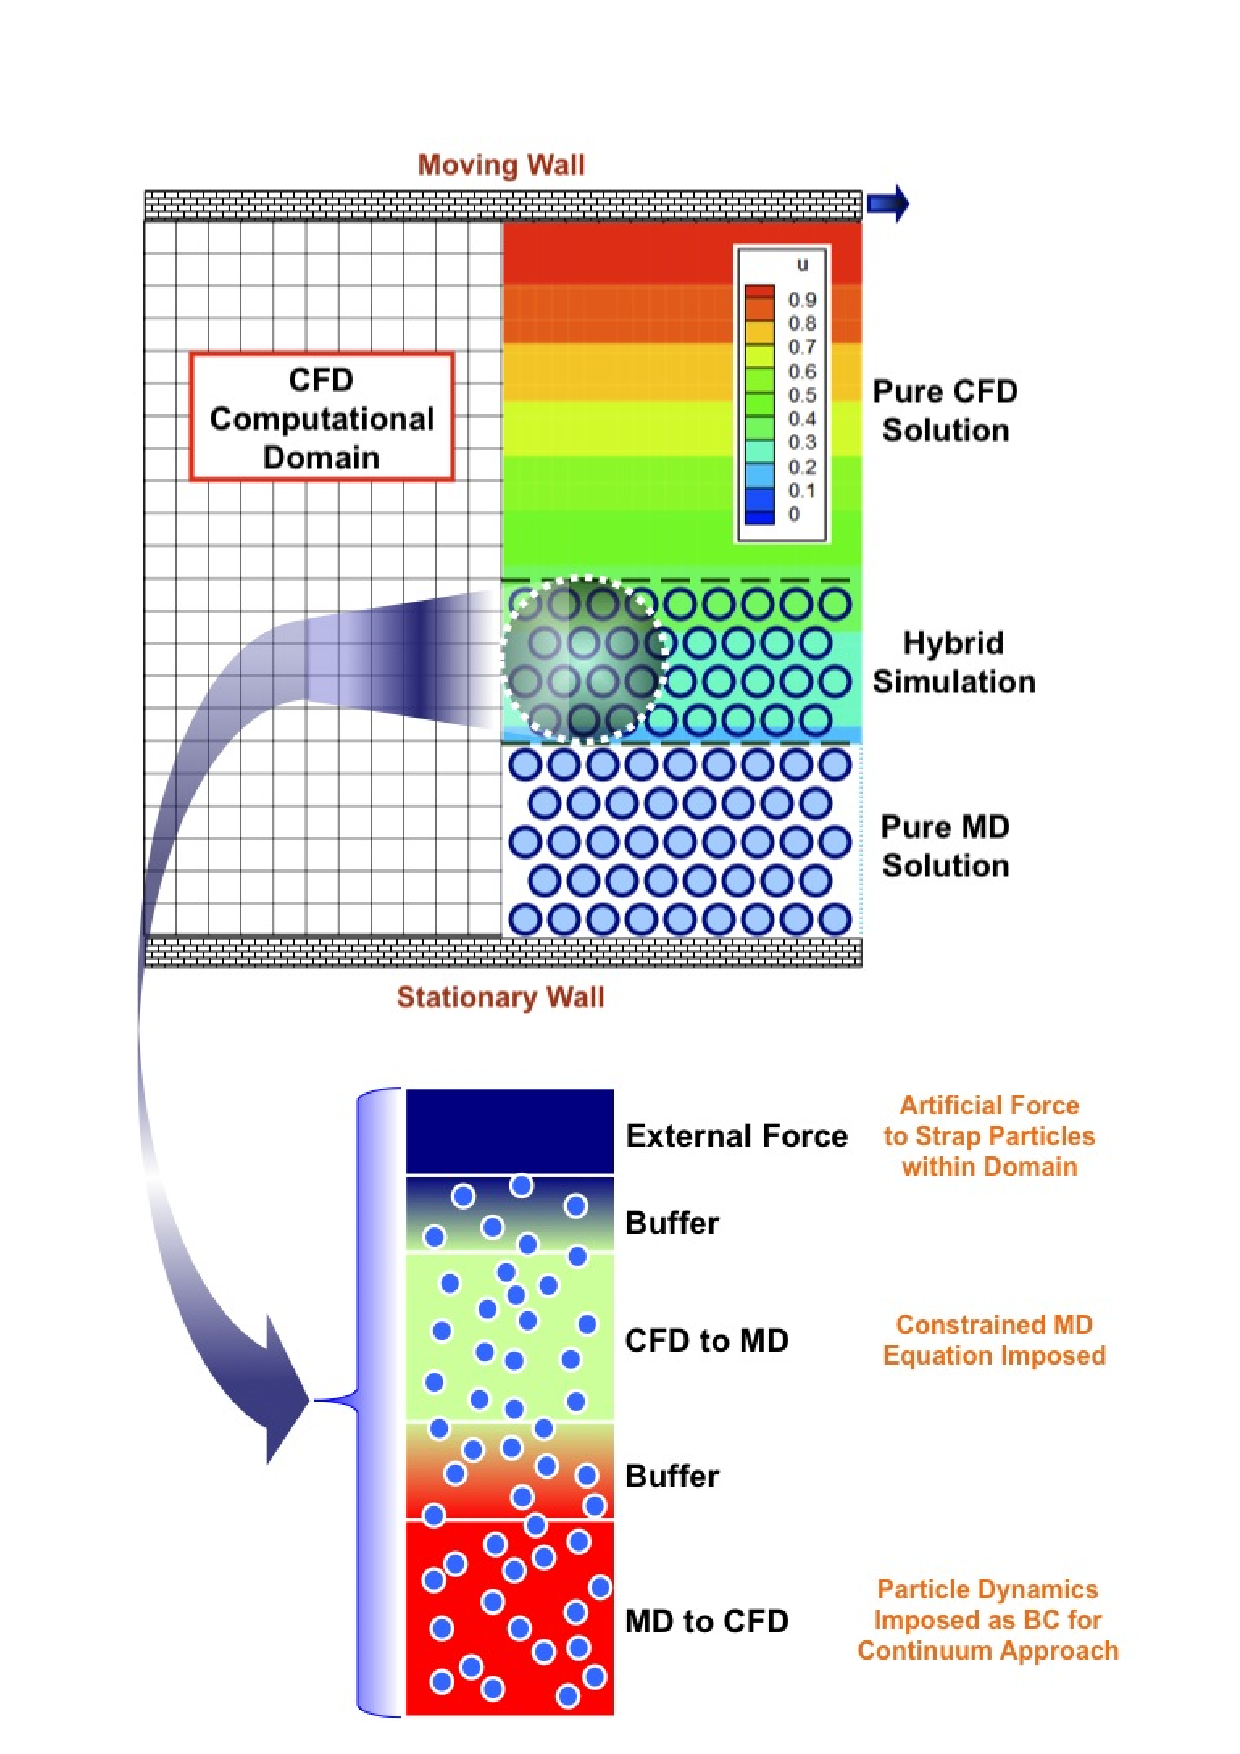
\includegraphics[scale=0.5]{fig1.pdf}
%\includegraphics[scale=0.3]{Couette7.pdf}
%\linebreak
\includegraphics[width=0.6\linewidth]{Couette7.pdf}
\vskip-0.2cm
\caption{Schematic Diagram of the Hybrid Domain with Detailed View of Overlapping Zone}
\label{Fig:Couette}
%\vspace{-1em}
\end{figure}
%%%%% FIGURE %%%%%



\section{IMPLEMENTATION OF HYBRID SCHEME ON CFD AND MD SOLVERS}

\subsection{Features of Baseline CFD and MD Codes}
Two-dimensional unsteady incompressible Navier-Stokes equations are chosen for governing equations to solve the nano-scale flow. In this work, we adopted the pseudo-compressibility method$^{\cite{PseudoCompressibility}}$ to form a hyperbolic system of equations which can be marched in pseudo-time. For time-accurate unsteady simulation, dual time stepping method is adopted and it is combined with the LU-SGS (Lower-Upper Symmetric Gauss-Seidel) scheme$^{\cite{LU-SGS}}$ for the implicit time integration. The inviscid fluxes are upwind-differenced using Osher's flux-difference splitting scheme$^{\cite{Osher}}$. Higher-order accurate solution can be gained by applying the MUSCL (Monotone Upstream-centered Schemes for Conservation Laws) approach on inviscid flux calculation and second-order central differencing on viscous fluxes.


Molecular dynamics (MD) is a specified computer simulation method for molecular systems, including microscopic details of a system and macroscopic statistical properties, which are the properties of the atoms, the interactions between particles, molecular characteristics, structure of molecules, transport phenomena etc.$^{\cite{Allen}}$ In molecular dynamics, an initial velocity is assigned to each atom, and Newton's laws are employed at the atomic level to propagate the system's motion through time evolution. the potential energy can be written as the sum of pairwise interactions of particles such as commonly using the Lennard-Jones (12-6) potential. The time integration algorithm is required to integrate the equation of motion of the interacting particles and computing molecular trajectories, one of most common velocity Verlet algorithm is employed to compute the simulation.
In this work,  the MD simulations were performed by using the modified version of Large Atomic Molecular Massively Parallel Simulator(LAMMPS). It is the classical molecular dynamics open software written in C++ and developed by Sandia National Labs $\underline{(http://lammps.sandia.gov/)}$.



\subsection{Implementation of Hybrid Scheme}
Additional change made on CFD code is the implementation of overlapping scheme, in the same way as Chimera overset mesh$^{\cite{Chimera}}$. That is, pure MD region is declared as holes and MD boundary layers are treated as fringe cells. On the other hands, MD code experiences a lot of change to implement hybrid scheme. First, the external force should be imposed to prevent leaving particles from the control domain and the force is applied its perpendicular relative position of uppermost MD layer$^{\cite{Nie},\cite{Yen},\cite{Wang}}$. Also, imposing macroscopic information on the fine grained microscopic domain is very difficult, thus requires artificial intervention to maintain mass and momentum conservation. The classical MD equation of motion can be generalized to obtain constraint by adopting the fluctuation in acceleration of each particles and the continuum velocity and the mean microscopic velocity from MD over control domain provide the synchronization of the mass and momentum consistency$^{\cite{Nie},\cite{Yen}}$. Finally, both codes have the file interface for the information exchange in hybrid region, where each writes the velocity profile of overlapping region, waits for its counterpart's velocity data and receive the data as a boundary condition in the overlap region.

For coupling in time domain, we adopted the synchronized coupling approach. Briefly, CFD and MD solvers do information exchange at the same time level in time domain and independently advance to the next exchange point without a large cost on waiting. Compared to sequential coupling approach, this method is clearly far more cost-effective. On the other hand, a slight time-lagging in hybrid boundary is inevitable.



\section{NUMERICAL RESULTS}

The first problem is the Couette flow simulation, which have been in wide use for the validation of a hybrid CFD-MD solver.$^{\cite{Nie},\cite{Yen}}$ We start from the validation case, which has 52$\sigma$ distance between two parallel plates and upper wall velocity is ${\sigma}/{\tau}$. We assume liquid argon particles are filled in the domain and both walls have artificial properties which is the same as those of liquid argon. Characteristic length of liquid argon is ${\sigma}=3.405{\times}10^{-10}$ and time scale is $\tau=2.2{\times}10^{-12}$. Density is $0.81m{\sigma}^{-3}$, which means 0.81 atoms are included in the characteristic volume. Of the fluid domain, 10$\sigma$ at the bottom is pure MD region, next 16$\sigma$ is hybrid zone and pure CFD region is upper half of the fluid domain.

MD solution inherently describes the Brownian movement of particles, which becomes a noise in continuum solution. Thus, the first thing to do for coupled simulation is to decide coupling conditions including layer size, sampling duration, sampling interval and MD timescale, which defines the scale and pattern of noise. We conducted pure MD simulations on stationary flow and checked the scale of noise, as seen from Fig.~\ref{MD_Regular_Vel0}. Comparing two graphs, we cannot see much influence of MD timescale on noise if sampling duration is longer than 10$\tau$. In each simulation, solution tends to produce less noise with bigger layer size and smaller MD timescale in short sampling duration. All solutions converges to the specific strength (0.01$\sigma$/$\tau$) as we increase the sampling interval, which implies that this noise in hybrid boundary is unavoidable. From this test, we decide the coupling condition as $\Delta{t_{MD}}=5\times{10^{3}}$ with each layer size to be 2$\sigma$ (which is nearly equivalent to having 24 layer), sampling duration of 10$\tau$ and sampling interval is set up the double of sampling duration.

%
\begin{figure}[ht]
\centering
\includegraphics[width=0.4\linewidth]{MD_Regular_Vel0_5e-3.pdf}
\hskip 1cm
\includegraphics[width=0.4\linewidth]{MD_Regular_Vel0_1e-3.pdf}
\vskip-0.2cm
\caption{L2 Norm of Averaged Velocity with Different Layer Sizes and Sampling Duration, at $\Delta{t_{MD}}=5\times{10^{3}}$ (Left) and $\Delta{t_{MD}}=1\times{10^{3}}$ (Right)}
\label{MD_Regular_Vel0}
\end{figure}



Unsteady Couette flow profile by CFD, MD and hybrid simulations are presented in Fig.~\ref{Flat_Plate_Sol}. Pure CFD produces identically the same result as analytic solution and MD simulations also describes the same velocity profile, though some infinitesimal difference is observed. This verifies that CFD and MD represents the same flow physics. In hybrid simulation, the molecular vibration from MD solution causes the slight variation in hybrid solution. Also, a little time-lagging in the hybrid region is detected, which is due by the synchronized coupling approach. Nevertheless, the steady solution follows the same flow pattern as other approaches, which proves that the hybrid approach can accurately analyze the steady flow profile in micro-scaled systems.

%
\begin{figure}[ht]
\centering
\includegraphics[width=0.4\linewidth]{Flat_Plate_Sol1.pdf}
\hskip 1cm
\includegraphics[width=0.4\linewidth]{Flat_Plate_Sol2.pdf}
\vskip-0.2cm
\caption{Unsteady Couette Flow Profile by CFD, MD and Hybrid Methods}
\label{Flat_Plate_Sol}
\end{figure}



The same domain with coupling condition is applied to solve the Stokes boundary layer problem, as seen in Fig.~\ref{Stokes_Sol}. In this simulation, all conditions are identical to Couette flow simulation, except the upper wall has $u_{wall}(t)=({\sigma}/{\tau}){\times}sin(2{\pi}t/T)$. Period $T$ is set 200$\tau$. The solution shows that the oscillatory velocity profile by pure CFD and hybrid simulations are globally the same, while minor time-lagging solution is observed in hybrid boundary. though synchronized coupling approach produces minor time-lagging in hybrid boundary. This leaves us the necessity to improve synchronized coupling approach to be time-accurate.

%
\begin{figure}[ht]
\centering
\includegraphics[width=0.4\linewidth]{Stokes_Sol_1.pdf}
\hskip 1cm
\includegraphics[width=0.4\linewidth]{Stokes_Sol_2.pdf}
\vskip-0.2cm
\caption{Unsteady Flow Profile of Stokes Boundary Layer Problem}
\label{Stokes_Sol}
\end{figure}



\section{CONCLUSIONS}

In this paper, we have discussed two important issues (coupling condition setup and unsteady flow simulation) on hybrid CFD-MD approach. Coupling condition which calibrates artificial noise of velocity profile due to limited averaging space and time can be determined by pure MD simulation of stationary flow in the same system. Stationary flow simulation does not require high cost and gives us the amount of unavoidable system noise, which can be the standard of determining coupling condition. By applying our simulation package with determined coupling condition to micro-scale problems, we get globally accurate flow profile in both Couette flow simulation and Stokes boundary layer simulation. However, time-lagging effect on hybrid boundary is observed because of the use of synchronized coupling approach, which should be resolved for unsteady flow simulation.

%Still, we are struggling from some issues. Coupling strategy in time domain is one important topic. The synchronized coupling approach we adopted has the clear benefit in view of parallel performance, but it also produces time-lagging in hybrid boundary which costs accurate .



\section*{ACKNOWLEDGEMENT}
This work is part of the Cybertools (\underline {http://cybertools.loni.org/}) project and primarily funded by NSF/LEQSF (2007-10)-CyberRII-01.
%This work has also been made possible thanks to computer resources provided by LONI.


\begin{thebibliography}{99}
%\bibitem{Zienkiewicz} O. C. Zienkiewicz and R. C. Taylor, The finite element method, 4th Edition, \textit{McGraw Hill}, \textbf{Vol. I} (1989), \textbf{Vol. II} (1991).
%\bibitem{Idelsohn} S. Idelsohn and E. O\~nate, Finite element and finite volumes, Two good friends, \textit{Int. J. Num. Meth. Engng.}, \textbf{37}, 3323--3341 (1994).
%\bibitem{Abgrall} R. Abgrall, M. Ricchiuto, N. Villedieu, C. Tav\'e\ and H. Deconinck, Very High Order Residual Distribution On Triangular Grids, In proceedings of the \textit{European Conference on Computational Fluid Dynamics}, ECCOMAS CFD 2006, P. Wesseling, E. O\~nate and J. Periaux Eds., Egmond aan Zee, Netherlands, Paper n$^{\circ}$583 (2006)



\bibitem{Thompson} S.T. O'Connell and P.A. Thompson, Molecular Dynamics Continuum Hybrid Computations: a Tool for Studying Complex Fuid Flows, \textit{Phys. Rev. E.}, \textbf{500}, 55--64 {2004}.
\bibitem{Nie} X. B. Nie and S. Y. Chen, W. N. E and M. O. Robbins, A Continuum and Molecular Dynamics Hybrid Method for Micro- and Nano-Fluid Flow, \textit{J. Fluid Mech.}, \textbf{52}, R5792--R5795 {1995}.
\bibitem{Yen} T. H. Yen and C. Y. Soong and P. Y. Tzeng, Hybrid Molecular Dynamics-Continuum Simulation for Nano/Mesoscale Channel Flow, \textit{Microfluid Nanofluid}, \textbf{3}, 665--675 {2007}.
\bibitem{Steijl} R. Steijl and G. N. Barakos, Coupled Navier-Stokes--Molecular Dynamics Simulations using a Multi-physics Flow Simulation Framework, \textit{Int. J. Numer. Meth. Fluids}, \textbf{62}, 1081--1106, {2010}
\bibitem{CCGrid} S.-H. Ko, N. Kim, J. Kim, A. Thota and S. Jha, Efficient Runtime Environment for Coupled Multi-Physics Simulations: Dynamic Resource Allocation and Load-Balancing, In proceedings of \textit{The 10th IEEE/ACM International Symposium on Cluster, Cloud and Grid Computing (CCGrid 2010)}, Accepted for Publication {2010}

\bibitem{Flekkoy} E. G. Flekk$\phi$y, G. Wagner and J. Feder, Hybrid Model for Combined Particle and Continuum Dynamics., \textit{Europhys Lett.}, \textbf{52}, 271--276 {2000}.
\bibitem{Hadjicon2} N. G. Hadjiconstantinou, A. L. Garcia, M. Z. Bazant, G. He, Statistical Error in Particle Simulations of Hydrodynamic Phenomena., \textit{J. Comput. Phys.}, \textbf{187}, 274--297 {2003}.
\bibitem{Wang} Y. C. Wang, G. He, A Dynamic Coupling Model for Hybrid Atomistic-Continuum Computations., \textit{Chem. Eng. Sci.}, \textbf{62}, 3574--3579 {2007}.
\bibitem{Time_Mechanism} R. Delgado-Buscalioni and P. V. Coveney, Hybrid Molecular-Continuum Fluid Dynamics, \textit{Phil. Trans. R. Soc. Lond. A}, \textbf{362}, 1639--1654 {2004}.

\bibitem{PseudoCompressibility} S. E. Rosers and D. Kwak, An Upwind Differecing Scheme for the Time-Accurate Incompressible Navier-Stokes Equations, \textit{AIAA J.}, \textbf{28}, 253--262 {1990}.
\bibitem{LU-SGS} S. Yoon and A. Jameson, Lower-Upper Symmetric-Gauss-Seidel Method for the Euler and Navier-Stokes Equations, \textit{AIAA J.}, \textbf{26}, 1025--1026 {1988}.
\bibitem{Osher} M. M. Rai and S. R. Chakaravarthy, An Implicit Form of the Osher Upwind Scheme, \textit{AIAA J.}, \textbf{24}, 735--743 {1986}.
\bibitem{Allen} M. Allen and D. Tildesley, Computer Simulation of Liquids, \textit{Oxford. Science Publications }, {1987}.

\bibitem{Chimera} J. L. Steger, F. C. Dougherty and J. A. Benek, A Chimera Grid Scheme, \textit{Advances in Grid Generation}, \textbf{FED Vol. 5}, American Society of Mechanical Engineers, New York, 59?-69 {1983}.

\end{thebibliography}



\end{document}

